\documentclass[border=10pt]{standalone}
\usepackage{pgfplots}
\usepackage{tikz}
%\pgfplotsset{width=13cm,compat=1.8}

\begin{document}
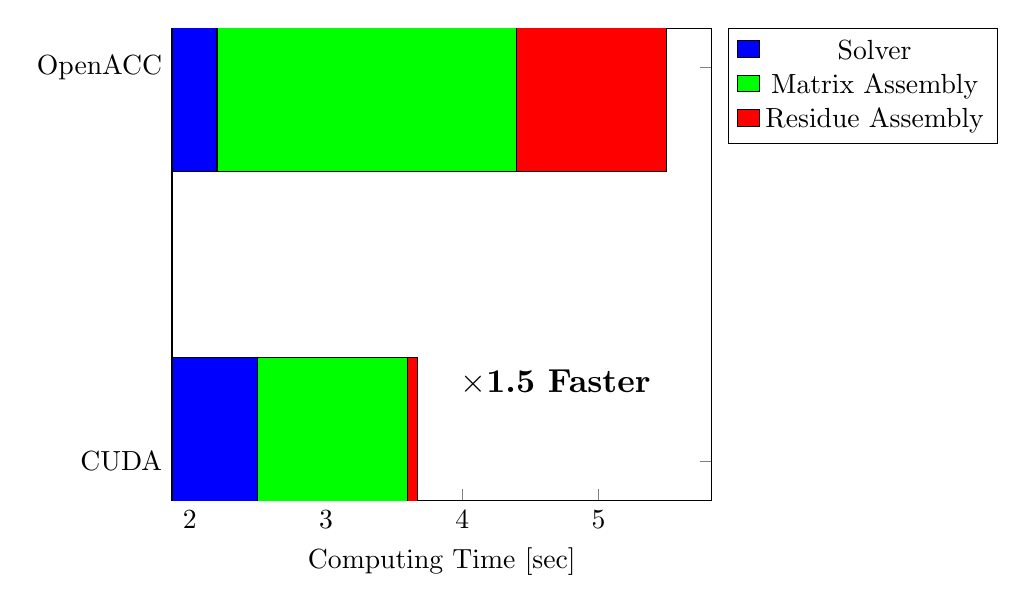
\begin{tikzpicture}[]
  \begin{axis}[scale=1.0,
      xbar stacked,
      bar width=75pt,
      %ybar=1pt,
      %width = 1cm,
      %enlargelimits=0.15,
      y=5cm,
      xlabel={Computing Time [sec]},
      symbolic y coords={CUDA,OpenACC},
      %y tick label style={at={axis cs:(0.5,0.5)}rotate=45, anchor=north east, inner sep=0mm},
      ytick=data,
      legend pos=outer north east,
      %legend cell align={left},
      legend style={fill=white},
      %legend style={at={(0.5,0.5)},fill=white,anchor=south west} 
      nodes near coords align={horizontal}
    ]
    \addplot[fill=blue,xbar] plot coordinates {
      (2.2,OpenACC) 
      (2.5,CUDA) 
    }; % sol cpu
    \addplot[fill=green,xbar] plot coordinates {
      (2.2,OpenACC)
      (1.1,CUDA)
    }; % mat
    \addplot[fill=red,xbar] plot coordinates {
      (1.1,OpenACC)
      (0.07,CUDA)
    }; % res cpu

    \legend{Solver, Matrix Assembly, Residue Assembly};
    %\draw[->, blue, line width=1mm] (-0.1cm,3cm) node[red, right] {$\times$\textbf{0.84}} -- ++(0,-1cm);
    %\draw[->, green, line width=1mm] (1.6cm,3cm) node[black, right] {$\times$\textbf{2}} -- ++(0,-1cm);
    %\draw[->, red, line width=1mm] (3.6cm,3cm) node[black, right] {$\times$\textbf{15.7}} -- ++(-1cm,-1cm);
    \node[scale=1.2] at (4.3cm,1.0cm) {$\times$\textbf{1.5 Faster}};
  \end{axis}
\end{tikzpicture}

% CPU
%ell_solve_cgpd 84251302
%assembly_mat   21056894
%assembly_rhs   2199559 
%total 107.5

% OpenACC
%ell_solve_cgpd 2158738         
%assembly_mat   2200091          
%assembly_rhs   1055412           
%total 5.5 

% CUDA
%ell_solve_cgpd 2543878 
%assembly_mat   1114047
%assembly_rhs   73563
%total 3.7

\end{document}
